\documentclass[conference]{IEEEtran}
\IEEEoverridecommandlockouts
\usepackage{cite}
\usepackage{amsmath,amssymb,amsfonts}
\usepackage{algorithmic}
\usepackage{algorithm}
\usepackage{graphicx}
\usepackage{textcomp}
\usepackage{xcolor}
\usepackage{booktabs}
\usepackage{tikz}
\usetikzlibrary{shapes.geometric,arrows.meta,positioning,calc,fit}

\def\BibTeX{{\rm B\kern-.05em{\sc i\kern-.025em b}\kern-.08em
    T\kern-.1667em\lower.7ex\hbox{E}\kern-.125emX}}

\begin{document}

\title{\LARGE Benchmarking Motion Gating for Wearable Heart-Rate Alerting}

\author{\IEEEauthorblockN{Student 1, \quad Student 2, \quad Student 3}
\IEEEauthorblockA{\textit{Department of Computer Science and Engineering} \\
\textit{Vel Tech Rangarajan Dr. Sagunthala R\&D Institute}, Chennai, India \\
email address}}

\maketitle

\begin{abstract}
Wearable cardiovascular monitors frequently combine signal quality heuristics with alerting thresholds to detect resting tachycardia. However, the incremental utility of multi-signal software trust scoring over simple kinematic motion gating is rarely benchmarked under pre-registered protocols. We present a reproducible, pre-registered fault-injection benchmark evaluating five alerting arms across fifteen ambulatory subjects from the public PPG-DaLiA dataset. To address natural event sparsity in healthy individuals, 112 labelled synthetic resting tachycardia episodes were injected into derived pulse-rate streams alongside two seeded telemetry fault regimes and raw optical noise. Evaluated in a strict leave-one-subject-out design with standard persistence and refractory hold-off, our primary hypothesis H1 was not supported. Kinematic motion gating drove nearly the entire reduction in false alerts per hour (reducing false alerts by roughly two-thirds to three-quarters relative to ungated personal baselines), while multi-attribute software trust scoring yielded no statistically significant improvement across any evaluated condition (paired differences were negligible and all ninety-five percent bootstrap confidence intervals spanned zero). Furthermore, aggressive software trust scoring degraded event recall under intense optical noise. Fixed population thresholding with persistence proved to be an unexpectedly robust baseline. Because events were synthetically injected and evaluated in healthy volunteers, these findings are exploratory and carry no clinical standing.
\end{abstract}

\begin{IEEEkeywords}
wearable sensors, photoplethysmography, heart-rate alerting, data quality, fault injection, negative result, reproducibility
\end{IEEEkeywords}

\section{Introduction}
Ambulatory continuous monitoring with consumer and medical-grade wearables offers substantial promise for early arrhythmia detection. However, wrist photoplethysmography (PPG) is acutely vulnerable to motion artifacts, optical decoupling, transmission dropouts, and flatline sensor lockups. When raw optical or derived telemetry signals degrade, alerting systems frequently emit spurious clinical notifications. In home monitoring and clinical telemetry alike, high false-alert frequencies precipitate severe alarm fatigue, inducing desensitization and compromising user adherence \cite{ref_alarm_fatigue}.

To prevent spurious alarms, modern digital health frameworks deploy complex signal quality indices (SQIs) and multi-component trust heuristics that penalize missing samples, flag frozen sensor values, and bound rate-of-change dynamics. Despite their architectural prevalence, the isolated incremental utility of multi-component software trust scores over straightforward kinematic stillness gating (e.g., Euclidean Norm Minus One, ENMO) has not been demonstrated in pre-registered, cross-validated benchmarks. Many prior evaluations suffer from train-test leakage, post-hoc hyperparameter selection, or lack of minimal baseline comparators.

This paper reports a rigorous, pre-registered fault-injection benchmark for wearable heart-rate alerting. Our contributions are:
\begin{enumerate}
    \item \textbf{Open Benchmarking Framework:} A fully reproducible pipeline formalizing an eight-type fault taxonomy (clean, gaps, stale values, duplicates, spikes, drift, scaling errors, and raw optical noise) evaluated across 31.25 hours of multi-activity ambulatory recordings.
    \item \textbf{Causal Leave-One-Subject-Out (LOSO) Evaluation:} Five distinct alerting arms evaluated with strict data quarantine, separating training folds from held-out evaluation subjects.
    \item \textbf{Rigorous Negative Finding:} Empirical refutation of pre-registered hypothesis $H_1$, showing that kinematic motion gating delivers 67.9\%--74.2\% false alert reduction, whereas multi-attribute software trust scoring provides no statistically detectable incremental benefit ($p \ge 0.28$).
\end{enumerate}

\section{Literature Survey}
Wrist-based pulse rate monitoring relies on optical absorption changes in microvascular tissue beds \cite{ref_reiss_dalia, ref_charlton_roadmap}. Relative motion between sensor photodiodes and cutaneous capillary beds introduces severe motion artifacts that overlap spectrally with true cardiac fundamental frequencies \cite{ref_reiss_dalia, ref_troika}.

To isolate motion artifact and evaluate waveform integrity, numerous signal quality indices (SQIs) have been proposed, spanning statistical moments (skewness, kurtosis), spectral purity, and template cross-correlation \cite{ref_elgendi_sqi}. While SQIs achieve strong classification performance on stationary laboratory datasets, ambulatory evaluations reveal severe performance drops during daily locomotion \cite{ref_reiss_dalia, ref_charlton_roadmap}. In clinical deployments, uncertainty quantification and selective prediction frameworks, such as conformal prediction, provide distribution-free finite-sample guarantees that offer structured paths for principled abstention \cite{ref_vazquez_conformal}. Table~\ref{tab:lit_comparison} contrasts existing wearable alerting paradigms with our pre-registered framework.

\begin{table}[htbp]
\caption{Comparative Overview of Wearable Alerting Paradigms}
\label{tab:lit_comparison}
\centering
\scriptsize
\begin{tabular}{|l|c|c|c|c|}
\hline
\textbf{Study / Paradigm} & \textbf{Pre-Reg.} & \textbf{Ablation} & \textbf{LOSO} & \textbf{Fault Inject.} \\
\hline
Deep PPG \cite{ref_reiss_dalia} & No & No & Yes & No \\
\hline
Optimal PPG SQI \cite{ref_elgendi_sqi} & No & No & No & No \\
\hline
PPG Roadmap \cite{ref_charlton_roadmap} & Review & N/A & N/A & N/A \\
\hline
Conformal Clinical UQ \cite{ref_vazquez_conformal} & Review & N/A & N/A & N/A \\
\hline
\textbf{This Benchmark} & \textbf{Yes} & \textbf{Yes} & \textbf{Yes} & \textbf{Yes} \\
\hline
\end{tabular}
\end{table}

\section{Dataset and Protocol}
\subsection{PPG-DaLiA Dataset}
We evaluate on the public PPG-DaLiA benchmark (UCI ID 495, CC BY 4.0) \cite{ref_reiss_dalia}. The dataset comprises 15 healthy subjects undergoing 2.5 hours of authentic daily activities (Table~\ref{tab:dataset}). Reference heart rates are derived from gold-standard chest ECG. Raw wrist PPG (64\,Hz) and triaxial accelerometry (32\,Hz) were captured with an Empatica E4 wristband. Strict quarantine was maintained: chest ECG reference was isolated solely for ground truth evaluation and was inaccessible to alerting arms.

\begin{table}[htbp]
\caption{PPG-DaLiA Benchmark Dataset Summary \cite{ref_reiss_dalia}}
\label{tab:dataset}
\centering
\scriptsize
\begin{tabular}{lp{4.8cm}}
\toprule
\textbf{Attribute} & \textbf{Specification} \\
\midrule
Subjects & $N = 15$ healthy individuals (7M, 8F, age 21--55, mean 30.6) \\
Protocol Duration & $\approx 2.5$\,h per subject ($31.25$ total ambulatory hours) \\
Activities & Sitting, Walking, Stairs, Cycling, Driving, Lunch, Soccer \\
Wrist Sensors & Empatica E4 (BVP: 64\,Hz, 3D ACC: 32\,Hz, GSR/Temp: 4\,Hz) \\
Reference Standard & Chest ECG (RespiBAN Professional, 700\,Hz) \\
Quarantine & Chest ECG strictly quarantined from alerting arms \\
\bottomrule
\end{tabular}
\end{table}


\subsection{Labelled Synthetic Tachycardia Injection}
Because natural resting tachycardia was virtually absent in this healthy volunteer cohort (manifesting in only 3 of 15 subjects), evaluating sensitivity on raw data is statistically uninformative. Per Amendment 2, we injected 112 labelled synthetic resting tachycardia episodes into derived pulse-rate streams during verified low-motion windows ($\text{ENMO}_{10\text{s}} \le 0.05$\,g). Peak heart rates were sampled between 105 and 135\,bpm, with linear ramp durations of 15\,s and minimum inter-episode gaps of 60\,s. To respect participant baseline heart rates $HR_{\text{base}}$, lower and upper ramp bounds were adaptively adjusted: $r_{\text{lo}} = \max(2.0, (105 - HR_{\text{base}})/15)$, $r_{\text{hi}} = \min(4.0, (135 - HR_{\text{base}})/15)$, with plateau peak heart rate clamped to $[105.0, 135.0]$\,bpm.

\subsection{Seeded Fault Regimes}
Sensor telemetry faults were simulated under two pre-specified schedules alongside an optical corruption condition (Table~\ref{tab:fault_taxonomy}):
\begin{itemize}
    \item \textbf{Condition 0 (No-Fault):} Clean ambulatory background.
    \item \textbf{Regime A (Low Duty, $\approx 10\%$ faulted time):} Sporadic gaps, stale values, duplicates, and slow drift (seed 42).
    \item \textbf{Regime B (Nominal Duty, $\approx 25\text{--}30\%$ faulted time):} Frequent dropouts, prolonged flatlines, and scale errors (seed 42).
    \item \textbf{F7 (High-Motion Optical Noise):} Additive Gaussian noise continuously modulated by wrist 3D acceleration injected into raw 64\,Hz BVP at SNR $+5.0$\,dB prior to Step 3a spectral estimation.
\end{itemize}

\begin{table}[htbp]
\caption{Fault Taxonomy and Seeded Regimes (Protocol Amendment 3)}
\label{tab:fault_taxonomy}
\centering
\scriptsize
\begin{tabular}{|l|p{3.3cm}|c|c|}
\hline
\textbf{Fault ID} & \textbf{Mechanism \& Parameter} & \textbf{Reg. A} & \textbf{Reg. B} \\
\hline
F0\_CLEAN & Ambient background & 28.09\,h & 21.67\,h \\
\hline
F1\_GAPS & Packet dropout (5--15\,s NaN) & 0.94\,h & 3.15\,h \\
\hline
F2\_STALE & Sensor freeze (10--30\,s constant) & 0.62\,h & 1.58\,h \\
\hline
F3\_DUPL & Repeated packets (burst 2--5) & 0.62\,h & 1.56\,h \\
\hline
F4\_SPIKE & Sudden jumps ($\pm 30$--$60$\,bpm) & 0.07\,h & 0.21\,h \\
\hline
F5\_DRIFT & Slow ramp ($+0.2$\,bpm/s trend) & 0.45\,h & 1.55\,h \\
\hline
F6\_UNIT & Scale error ($0.5\times$ or $2.0\times$) & 0.48\,h & 1.56\,h \\
\hline
F7\_OPTICAL & Motion noise ($\text{SNR}=+5$\,dB, 64\,Hz) & Standalone & Standalone \\
\hline
\end{tabular}
\end{table}


\section{System Architecture}
The experimental harness and interactive replay lab were implemented as a modular full-stack application (Fig.~\ref{fig:arch}). The front-end is a React Progressive Web Application (PWA) aligned with Figma interactive specifications, featuring live telemetry inspection, threshold tuning, and an interactive benchmark dashboard. In terms of product requirements (PRD), core streaming telemetry and visual replay are operational. Requirement FR-04 (data quality checks) is currently partial: anomaly flags (missing data, flatlines, physiological bounds) are active, while automated exclusion from inference is pending. Modules FR-06 (guided symptom-risk questionnaire with user review step) and FR-07 (explanation with prediction uncertainty) are planned for future increments. The back-end is powered by FastAPI and SQLite, incorporating the core \texttt{vitasense.quality} engine, replay caches, and LLM assistant routing with rule-based safety fallbacks.

\begin{figure}[htbp]
\centering
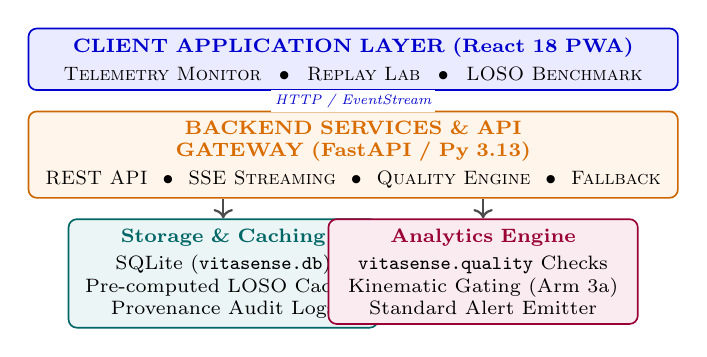
\begin{tikzpicture}[
    layer/.style={rectangle, draw=#1!80!black, fill=#1!8, rounded corners=3pt, font=\scriptsize, align=center, inner sep=3.5pt, line width=0.6pt},
    arr/.style={-{Stealth[length=1.5mm, width=1.1mm]}, thick, color=black!70}
]
\node[layer=blue, text width=3.15in] (ui) {
    \textbf{\textcolor{blue!80!black}{CLIENT APPLICATION LAYER (React 18 PWA)}}\\[2pt]
    \textsc{Telemetry Monitor} $\;\bullet\;$ \textsc{Replay Lab} $\;\bullet\;$ \textsc{LOSO Benchmark}
};

\node[layer=orange, below=0.25cm of ui, text width=3.15in] (api) {
    \textbf{\textcolor{orange!85!black}{BACKEND SERVICES \& API GATEWAY (FastAPI / Py 3.13)}}\\[2pt]
    \textsc{REST API} $\;\bullet\;$ \textsc{SSE Streaming} $\;\bullet\;$ \textsc{Quality Engine} $\;\bullet\;$ \textsc{Fallback}
};

\node[layer=teal, below=0.25cm of api, xshift=-1.65cm, text width=1.45in] (db) {
    \textbf{\textcolor{teal!80!black}{Storage \& Caching}}\\[2pt]
    SQLite (\texttt{vitasense.db})\\
    Pre-computed LOSO Caches\\
    Provenance Audit Logs
};

\node[layer=purple, below=0.25cm of api, xshift=1.65cm, text width=1.45in] (engine) {
    \textbf{\textcolor{purple!80!black}{Analytics Engine}}\\[2pt]
    \texttt{vitasense.quality} Checks\\
    Kinematic Gating (Arm 3a)\\
    Standard Alert Emitter
};

\draw[arr, <->] (ui.south) -- (api.north) node[midway, fill=white, inner sep=1.5pt, font=\tiny\itshape, text=blue!80!black] {HTTP / EventStream};
\draw[arr, ->] (api.south -| db) -- (db.north);
\draw[arr, ->] (api.south -| engine) -- (engine.north);
\end{tikzpicture}
\caption{Visual Architecture: VitaSense full-stack telemetry and benchmark application.}
\label{fig:arch}
\end{figure}

\section{Methods and Algorithms}
\subsection{Evaluated Alerting Arms and Pipeline}
The research pipeline processes raw sensor streams into calibrated, causal alerts without future peeking (Fig.~\ref{fig:pipeline}). We benchmark five causal alerting arms (Fig.~\ref{fig:arms}):
\begin{enumerate}
    \item \textbf{Arm 1 (Fixed Population Cutoff):} Standard clinical threshold $\tau_{\text{pop}} \in \{100, 110, 120, 125, 130\}$\,bpm.
    \item \textbf{Arm 2 (Personal Baseline with Shrinkage):} Dynamic cutoff $\tau_i(t) = \max(\tau_{\text{floor}}, \hat{\mu}_i(t) + k \cdot \hat{\sigma}_i(t))$ regularized toward training-population priors $(\mu_{\text{pop}}, \sigma_{\text{pop}})$ via empirical Bayes shrinkage $\kappa$ (Algorithm~\ref{alg:causal_baseline}).
    \item \textbf{Arm 3a (Kinematic Motion Gating):} Arm 2 personal baseline paired with a stillness gate: alert triggers if and only if $HR(t) > \tau_i(t)$ and $\text{ENMO}_{10\text{s}}(t) \le \theta_{\text{rest}}$.
    \item \textbf{Arm 3b (Multi-Attribute Trust Score Gating):} Arm 2 baseline gated by software trust score: alert triggers if and only if $HR(t) > \tau_i(t)$ and $S_{\text{trust}}(t) \ge \theta_{\text{trust}}$.
    \item \textbf{Arm 3b-noMotion (Trust Ablation):} Arm 3b with kinematic motion term ablated ($w_{\text{mot}} = 0$).
\end{enumerate}

\begin{figure}[htbp]
\centering
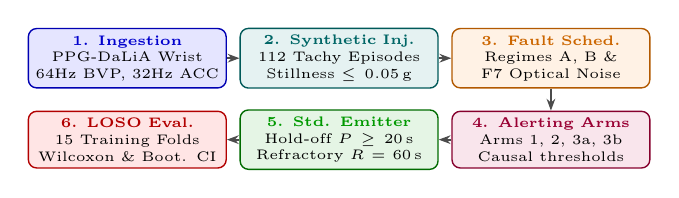
\begin{tikzpicture}[
    stepnode/.style={rectangle, draw=#1!70!black, fill=#1!10, rounded corners=3pt, font=\tiny, align=center, inner sep=2.5pt, line width=0.5pt, text width=0.92in},
    arr/.style={-{Stealth[length=1.5mm, width=1.1mm]}, thick, color=black!70}
]
\node[stepnode=blue] (s1) {\textbf{\textcolor{blue!80!black}{1. Ingestion}}\\PPG-DaLiA Wrist\\64Hz BVP, 32Hz ACC};
\node[stepnode=teal, right=0.16cm of s1] (s2) {\textbf{\textcolor{teal!80!black}{2. Synthetic Inj.}}\\112 Tachy Episodes\\Stillness $\le 0.05$\,g};
\node[stepnode=orange, right=0.16cm of s2] (s3) {\textbf{\textcolor{orange!80!black}{3. Fault Sched.}}\\Regimes A, B \&\\F7 Optical Noise};

\node[stepnode=purple, below=0.28cm of s3] (s4) {\textbf{\textcolor{purple!80!black}{4. Alerting Arms}}\\Arms 1, 2, 3a, 3b\\Causal thresholds};
\node[stepnode=green!60!black, left=0.16cm of s4] (s5) {\textbf{\textcolor{green!60!black}{5. Std. Emitter}}\\Hold-off $P \ge 20$\,s\\Refractory $R = 60$\,s};
\node[stepnode=red, left=0.16cm of s5] (s6) {\textbf{\textcolor{red!70!black}{6. LOSO Eval.}}\\15 Training Folds\\Wilcoxon \& Boot. CI};

\draw[arr] (s1) -- (s2);
\draw[arr] (s2) -- (s3);
\draw[arr] (s3) -- (s4);
\draw[arr] (s4) -- (s5);
\draw[arr] (s5) -- (s6);
\end{tikzpicture}
\caption{Visual Pipeline: Pre-registered fault injection and LOSO benchmarking.}
\label{fig:pipeline}
\end{figure}

\begin{figure}[htbp]
\centering
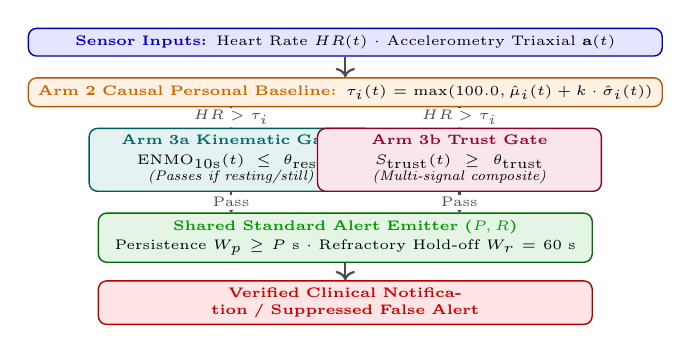
\begin{tikzpicture}[
    box/.style={rectangle, draw=#1!70!black, fill=#1!10, rounded corners=3pt, font=\tiny, align=center, inner sep=2.5pt, line width=0.5pt},
    arr/.style={-{Stealth[length=1.5mm, width=1.1mm]}, thick, color=black!70}
]
\node[box=blue, text width=3.1in] (inp) {\textbf{\textcolor{blue!80!black}{Sensor Inputs:}} Heart Rate $HR(t)$ $\cdot$ Accelerometry Triaxial $\mathbf{a}(t)$};
\node[box=orange, below=0.26cm of inp, text width=3.1in] (tau) {\textbf{\textcolor{orange!80!black}{Arm 2 Causal Personal Baseline:}} $\tau_i(t) = \max(100.0, \hat{\mu}_i(t) + k \cdot \hat{\sigma}_i(t))$};

\node[box=teal, below=0.26cm of tau, xshift=-1.45cm, text width=1.35in] (g_kin) {
    \textbf{\textcolor{teal!80!black}{Arm 3a Kinematic Gate}}\\[1pt]
    $\text{ENMO}_{10\text{s}}(t) \le \theta_{\text{rest}}$\\
    \textit{(Passes if resting/still)}
};

\node[box=purple, below=0.26cm of tau, xshift=1.45cm, text width=1.35in] (g_tr) {
    \textbf{\textcolor{purple!80!black}{Arm 3b Trust Gate}}\\[1pt]
    $S_{\text{trust}}(t) \ge \theta_{\text{trust}}$\\
    \textit{(Multi-signal composite)}
};

\node[box=green!60!black, below=0.26cm of $(g_kin.south)!0.5!(g_tr.south)$, text width=2.4in] (emit) {
    \textbf{\textcolor{green!60!black}{Shared Standard Alert Emitter ($P, R$)}}\\[1pt]
    Persistence $W_p \ge P$ s $\cdot$ Refractory Hold-off $W_r = 60$ s
};

\node[box=red, below=0.22cm of emit, text width=2.4in] (out) {
    \textbf{\textcolor{red!80!black}{Verified Clinical Notification / Suppressed False Alert}}
};

\draw[arr, ->] (inp.south) -- (tau.north);
\draw[arr, ->] (tau.south -| g_kin) -- (g_kin.north) node[midway, fill=white, inner sep=1pt, font=\tiny\bfseries] {$HR > \tau_i$};
\draw[arr, ->] (tau.south -| g_tr) -- (g_tr.north) node[midway, fill=white, inner sep=1pt, font=\tiny\bfseries] {$HR > \tau_i$};
\draw[arr, ->] (g_kin.south) -- (emit.north -| g_kin.south) node[midway, fill=white, inner sep=1pt, font=\tiny] {Pass};
\draw[arr, ->] (g_tr.south) -- (emit.north -| g_tr.south) node[midway, fill=white, inner sep=1pt, font=\tiny] {Pass};
\draw[arr, ->] (emit.south) -- (out.north);
\end{tikzpicture}
\caption{Visual Decision Flow: Causal alerting logic and dual gating pathways.}
\label{fig:arms}
\end{figure}

\subsection{Shared Standard Alert Emitter}
To ensure rigorous cross-arm comparability, all arms feed instantaneous binary triggers into a shared \texttt{StandardAlertEmitter} (Algorithm~\ref{alg:emitter}). Alerts fire if and only if triggering conditions hold continuously for $W_p = P / \text{step}$ windows ($P \in \{10, 20, 30\}$\,s). Emitted alerts enforce a mandatory refractory hold-off of $W_r = R / \text{step}$ windows ($R = 60$\,s).

\begin{algorithm}[htbp]
\caption{Synthetic Tachycardia Injection \& Fault Schedule}
\label{alg:synth_fault}
\scriptsize
\begin{algorithmic}[1]
\REQUIRE Pulse rate $HR$, motion $\text{ENMO}$, seed $S = 42$, regime $\mathcal{R}$
\STATE Identify resting blocks $\mathcal{B} = \{[t_s, t_e] \mid \text{ENMO}[t] \le 0.05\,\text{g}, \text{dur} \ge 80\,\text{s}\}$
\FOR{episode $j = 1$ to $N_{\text{tachy}}$ (sample without overlap, gap $\ge 60$\,s)}
    \STATE Sample target plateau $HR_{\text{peak}} \sim \mathcal{U}(105, 135)$\,bpm
    \STATE Compute adaptive ramp rates: $r \leftarrow (HR_{\text{peak}} - HR_{\text{base}})/15\,\text{s}$
    \STATE Inject 15\,s ramp, plateau (45--120\,s), 20\,s exponential decay
\ENDFOR
\IF{$\mathcal{R} \in \{\text{Regime A}, \text{Regime B}\}$}
    \STATE Sample non-overlapping fault intervals outside synthetic events
    \STATE Inject F1 (gaps), F2 (stale), F3 (dupl), F4 (spikes), F5 (drift), F6 (unit scale)
\ELSIF{$\mathcal{R} == \text{F7}$}
    \STATE Add optical Gaussian noise modulated by $\|\mathbf{a}(t)\|$ at $+5.0$\,dB SNR
\ENDIF
\RETURN Fault-injected stream $HR_{\text{faulted}}$ and episode ground truth
\end{algorithmic}
\end{algorithm}

\begin{algorithm}[htbp]
\caption{Causal Personal Baseline \& Trust Score Gating}
\label{alg:causal_baseline}
\scriptsize
\begin{algorithmic}[1]
\REQUIRE $HR$, $\text{ENMO}$, priors $\mu_{\text{pop}}, \sigma_{\text{pop}}$, grid $k, \kappa, \theta_{\text{rest}}, \theta_{\text{trust}}$
\FOR{window index $t = 0$ to $N-1$}
    \STATE $c \leftarrow \sum_{\tau=0}^{t-1} \mathbb{I}(\text{ENMO}[\tau] \le 0.05 \land \text{finite}(HR[\tau]))$
    \IF{$c > 1$}
        \STATE $\bar{x} \leftarrow \frac{1}{c} \sum_{\tau < t} HR[\tau], \quad s \leftarrow \text{std}_{\tau < t}(HR[\tau])$
    \ELSE
        \STATE $\bar{x} \leftarrow \mu_{\text{pop}}, \quad s \leftarrow \sigma_{\text{pop}}$
    \ENDIF
    \STATE $w \leftarrow \frac{c \cdot \Delta t / 3600}{c \cdot \Delta t / 3600 + \kappa}; \quad \hat{\mu} \leftarrow w \bar{x} + (1-w)\mu_{\text{pop}}; \quad \hat{\sigma} \leftarrow w s + (1-w)\sigma_{\text{pop}}$
    \STATE $\tau_i[t] \leftarrow \max(100.0, \hat{\mu} + k \cdot \hat{\sigma})$
    \STATE $S_{\text{gap}} \leftarrow 1 - 2 \cdot \text{nan\_ratio}; \quad S_{\text{stale}} \leftarrow \mathbb{I}(\text{var} \ge 10^{-6})$
    \STATE $S_{\text{phys}} \leftarrow \mathbb{I}(35 \le HR \le 220 \land |\Delta HR| \le 40)$
    \STATE $S_{\text{mot}} \leftarrow \text{clip}(1.0 - 0.60 \cdot (\text{ENMO} - 0.05)/0.25, 0.2, 1.0)$
    \STATE $S_{\text{trust}}[t] \leftarrow \text{clip}(S_{\text{gap}} \cdot S_{\text{stale}} \cdot S_{\text{phys}} \cdot S_{\text{mot}}, 0.0, 1.0)$
    \STATE $Cond_{\text{3a}}[t] \leftarrow (HR[t] > \tau_i[t]) \land (\text{ENMO}[t] \le \theta_{\text{rest}})$
    \STATE $Cond_{\text{3b}}[t] \leftarrow (HR[t] > \tau_i[t]) \land (S_{\text{trust}}[t] \ge \theta_{\text{trust}})$
    \STATE $Cond_{\text{3b-noMot}}[t] \leftarrow (HR[t] > \tau_i[t]) \land (S_{\text{gap}} \cdot S_{\text{stale}} \cdot S_{\text{phys}} \ge \theta_{\text{trust}})$
\ENDFOR
\end{algorithmic}
\end{algorithm}

\begin{algorithm}[htbp]
\caption{Standard Alert Emitter with Refractory Hold-off}
\label{alg:emitter}
\scriptsize
\begin{algorithmic}[1]
\REQUIRE Raw condition mask $C$, persistence $W_p = P / \Delta t$, refractory $W_r = R / \Delta t$
\STATE $run\_len \leftarrow 0, \quad ref\_cnt \leftarrow 0, \quad Alert \leftarrow \mathbf{0}$
\FOR{$t = 0$ to $N-1$}
    \IF{$ref\_cnt > 0$}
        \STATE $ref\_cnt \leftarrow ref\_cnt - 1$
    \ENDIF
    \IF{$C[t]$ is TRUE}
        \STATE $run\_len \leftarrow run\_len + 1$
        \IF{$run\_len \ge W_p$ \AND $ref\_cnt == 0$}
            \STATE $Alert[t] \leftarrow \text{TRUE}; \quad ref\_cnt \leftarrow W_r; \quad run\_len \leftarrow 0$
        \ENDIF
    \ELSE
        \STATE $run\_len \leftarrow 0$
    \ENDIF
\ENDFOR
\RETURN $Alert$
\end{algorithmic}
\end{algorithm}

\begin{table}[htbp]
\caption{Evaluated Parameter Grids (Amendment 4)}
\label{tab:parameter_grids}
\centering
\scriptsize
\begin{tabular}{lp{4.5cm}c}
\toprule
\textbf{Arm} & \textbf{Tuned Parameters} & \textbf{Refractory $R$} \\
\midrule
Arm 1 & \raggedright $\tau_{\text{pop}} \in \{100, 110, 120, 125, 130\}$\,bpm; $P \in \{10, 20, 30\}$\,s & 60\,s \\
Arm 2 & \raggedright $k \in \{2.0, 2.5, 3.0, 3.5, 4.0\}$; $\kappa \in \{0.5, 1.0, 2.0\}$\,h; $P \in \{10, 20, 30\}$\,s & 60\,s \\
Arm 3a & \raggedright $\theta_{\text{rest}} \in \{0.03, 0.05, 0.08\}$\,g; $P \in \{10, 20, 30\}$\,s & 60\,s \\
Arm 3b & \raggedright $\theta_{\text{trust}} \in \{0.60, 0.70, 0.80\}$; $P \in \{10, 20, 30\}$\,s & 60\,s \\
Arm 3b-noMot & \raggedright $\theta_{\text{trust}} \in \{0.60, 0.70, 0.80\}$; $P \in \{10, 20, 30\}$\,s & 60\,s \\
\bottomrule
\end{tabular}
\end{table}

\begin{table*}[t]
\caption{Leave-One-Subject-Out Combined Alerting Benchmark Results Across Conditions (alert counts archived in alert\_counts.csv)}
\label{tab:combined_metrics}
\centering
\footnotesize
\renewcommand{\arraystretch}{0.92}
\setlength{\tabcolsep}{6.0pt}
\begin{tabular}{|l|l|c|c|c|c|}
\hline
\textbf{Condition} & \textbf{Alerting Arm} & \textbf{Recall (\%)} & \textbf{FA/hr} & \textbf{Precision (\%)} & \textbf{$F_1$ Score} \\
\hline
Condition 0 (No-Fault)       & Arm 1 (Fixed)                        & \textbf{91.1} &  3.20 &  56.9 & 0.700 \\
                             & Arm 2 (Personal)                     &  80.4 &  5.69 &  42.8 & 0.558 \\
                             & Arm 3a (+Kinematic)                  &  80.4 &  1.47 &  74.3 & 0.772 \\
                             & Arm 3b (+Trust Score)                &  79.5 &  1.69 &  71.0 & 0.750 \\
                             & Arm 3b-noMotion                      &  79.5 &  2.91 &  58.8 & 0.676 \\
                             & Arm 4 (conformal)\textsuperscript{*} &  72.3 & \textbf{0.70} & \textbf{83.7} & \textbf{0.776} \\
\hline
Regime A (Low Duty $\approx 10\%$)   & Arm 1 (Fixed)                        & \textbf{91.1} &  3.58 &  54.1 & 0.679 \\
                             & Arm 2 (Personal)                     &  80.4 &  6.08 &  41.0 & 0.543 \\
                             & Arm 3a (+Kinematic)                  &  80.4 &  1.63 &  72.1 & \textbf{0.760} \\
                             & Arm 3b (+Trust Score)                &  79.5 &  1.82 &  69.4 & 0.741 \\
                             & Arm 3b-noMotion                      &  79.5 &  3.07 &  57.3 & 0.666 \\
                             & Arm 4 (conformal)\textsuperscript{*} &  62.5 & \textbf{0.67} & \textbf{82.1} & 0.710 \\
\hline
Regime B (Nominal $\approx 25\text{--}30\%$) & Arm 1 (Fixed)                        & \textbf{91.1} &  4.51 &  48.4 & 0.632 \\
                             & Arm 2 (Personal)                     &  75.9 &  7.16 &  35.8 & 0.487 \\
                             & Arm 3a (+Kinematic)                  &  75.9 &  2.30 &  63.5 & \textbf{0.691} \\
                             & Arm 3b (+Trust Score)                &  75.0 &  2.37 &  62.2 & 0.680 \\
                             & Arm 3b-noMotion                      &  75.0 &  3.61 &  51.9 & 0.614 \\
                             & Arm 4 (conformal)\textsuperscript{*} &  55.4 & \textbf{0.70} & \textbf{79.0} & 0.651 \\
\hline
F7 (High-Motion BVP Noise)   & Arm 1 (Fixed)                        & \textbf{92.0} &  3.07 &  57.7 & \textbf{0.709} \\
                             & Arm 2 (Personal)                     &  64.3 &  4.61 &  41.0 & 0.501 \\
                             & Arm 3a (+Kinematic)                  &  64.3 &  1.57 &  67.1 & 0.657 \\
                             & Arm 3b (+Trust Score)                &  58.0 &  1.28 &  69.2 & 0.631 \\
                             & Arm 3b-noMotion                      &  58.0 &  2.05 &  58.4 & 0.582 \\
                             & Arm 4 (conformal)\textsuperscript{*} &  54.5 & \textbf{0.35} & \textbf{88.2} & 0.673 \\
\hline
\multicolumn{6}{l}{\scriptsize *\textit{Pre-specified in Amendment 3, implemented after other arms' results were seen.}} \\
\hline
\end{tabular}
\end{table*}


\section{Experimental Setup}
\subsection{Leave-One-Subject-Out (LOSO) Cross-Validation}
Hyperparameters were tuned strictly within 15 LOSO training folds (Algorithm~\ref{alg:loso_scoring}). For each test subject $s \in \{1\dots 15\}$, candidate configurations were evaluated across the 14 training subjects pooled. The pre-specified selection rule chooses the parameter vector achieving $\ge 85\%$ training recall while minimizing false alerts per hour ($\text{FA/hr}$). If no parameter setting reaches $85\%$ recall, the pre-registered fallback rule selects the setting maximizing training recall.

\begin{algorithm}[htbp]
\caption{LOSO Grid Tuning, Fallback Rule, and Dual Scoring}
\label{alg:loso_scoring}
\scriptsize
\begin{algorithmic}[1]
\REQUIRE Training folds $\mathcal{S}_{\text{train}}$, test subject $s_{\text{test}}$, parameter grid $\Theta$
\FOR{$\theta \in \Theta$}
    \STATE Evaluate pooled training recall $\text{Rec}_{\text{train}}(\theta)$ and $\text{FA/hr}_{\text{train}}(\theta)$
\ENDFOR
\STATE $\mathcal{V} \leftarrow \{\theta \in \Theta \mid \text{Rec}_{\text{train}}(\theta) \ge 0.85\}$
\IF{$\mathcal{V} \neq \emptyset$}
    \STATE $\theta^* \leftarrow \arg\min_{\theta \in \mathcal{V}} \text{FA/hr}_{\text{train}}(\theta)$ \COMMENT{Primary selection rule}
\ELSE
    \STATE $\theta^* \leftarrow \arg\max_{\theta \in \Theta} \text{Rec}_{\text{train}}(\theta)$ \COMMENT{Fallback selection rule}
\ENDIF
\STATE Run chosen arm with $\theta^*$ on $s_{\text{test}}$ to yield alert mask $A$
\STATE $\text{TP} \leftarrow \sum_{j} \mathbb{I}(\exists t \in [t_{s,j}, t_{e,j}] : A[t] == \text{TRUE})$
\STATE $\text{Recall} \leftarrow \text{TP} / N_{\text{injected}}$
\STATE $\text{Clean FA} \leftarrow \sum_{t} \mathbb{I}(A[t] == \text{TRUE} \land t \notin \mathcal{T}_{\text{injected}} \land t \notin \mathcal{T}_{\text{natural} \pm 30\text{s}})$
\STATE $\text{FA/hr} \leftarrow \text{Clean FA} / T_{\text{non-event hours}}$
\RETURN Test performance $(\text{Recall}, \text{FA/hr})$
\end{algorithmic}
\end{algorithm}

\subsection{Evaluation Metrics and Paired Statistics}
Scoring evaluates event-level recall (detecting injected episodes within $[t_{\text{start}}, t_{\text{end}}]$) alongside alert-level clean false alerts per hour ($\text{FA/hr}$), precision on non-event periods, and $F_1$ score. The primary statistical hypothesis test compares paired per-subject differences ($\Delta = \text{Arm 3b} - \text{Arm 3a}$) using the two-sided Wilcoxon signed-rank test ($\alpha = 0.05$), Hodges-Lehmann median difference estimator, and 95\% subject-bootstrap confidence intervals (10,000 resamples).

\begin{figure}[htbp]
\centering
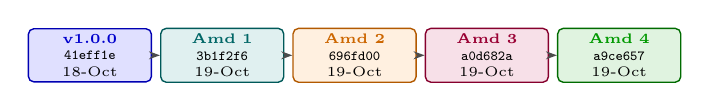
\begin{tikzpicture}[
    milestone/.style={rectangle, draw=#1!70!black, fill=#1!12, rounded corners=2pt, font=\tiny, align=center, inner sep=2pt, line width=0.5pt, text width=0.56in},
    arr/.style={-{Stealth[length=1.4mm, width=1.0mm]}, thick, color=black!70}
]
\node[milestone=blue] (v1) {\textbf{\textcolor{blue!80!black}{v1.0.0}}\\\texttt{41eff1e}\\18-Oct};
\node[milestone=teal, right=0.10cm of v1] (a1) {\textbf{\textcolor{teal!80!black}{Amd 1}}\\\texttt{3b1f2f6}\\19-Oct};
\node[milestone=orange, right=0.10cm of a1] (a2) {\textbf{\textcolor{orange!80!black}{Amd 2}}\\\texttt{696fd00}\\19-Oct};
\node[milestone=purple, right=0.10cm of a2] (a3) {\textbf{\textcolor{purple!80!black}{Amd 3}}\\\texttt{a0d682a}\\19-Oct};
\node[milestone=green!60!black, right=0.10cm of a3] (a4) {\textbf{\textcolor{green!60!black}{Amd 4}}\\\texttt{a9ce657}\\19-Oct};

\draw[arr] (v1) -- (a1);
\draw[arr] (a1) -- (a2);
\draw[arr] (a2) -- (a3);
\draw[arr] (a3) -- (a4);
\end{tikzpicture}
\caption{Visual Timeline: Pre-registered protocol amendments and git provenance.}
\label{fig:timeline}
\end{figure}

\begin{figure*}[t]
\centering
\begin{minipage}{0.48\textwidth}
\centering
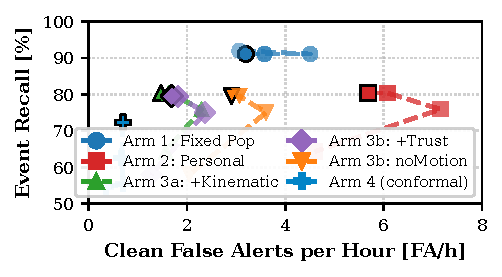
\includegraphics[width=0.98\linewidth, height=1.35in, keepaspectratio]{figures/fig_recall_vs_fahr.pdf}
\centerline{\footnotesize (a) Event Recall vs Clean False Alerts per Hour across Arms and Regimes}
\end{minipage}\hfill
\begin{minipage}{0.48\textwidth}
\centering
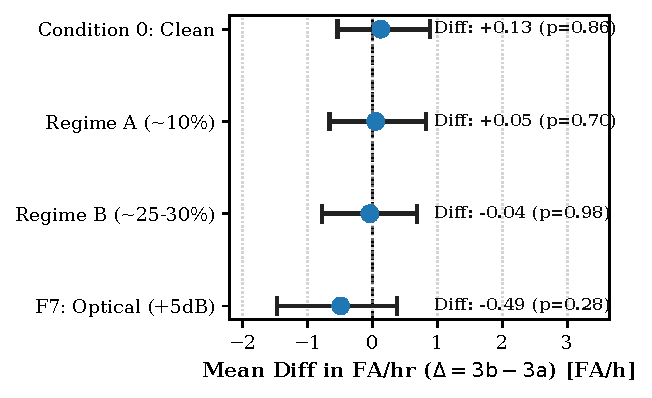
\includegraphics[width=0.98\linewidth, height=1.35in, keepaspectratio]{figures/fig_forest_plot_3b_vs_3a.pdf}
\centerline{\footnotesize (b) Paired Differences ($\Delta = \text{Arm 3b} - \text{Arm 3a}$) with 95\% Bootstrap CIs}
\end{minipage}

\vspace{0.08cm}

\begin{minipage}{0.48\textwidth}
\centering
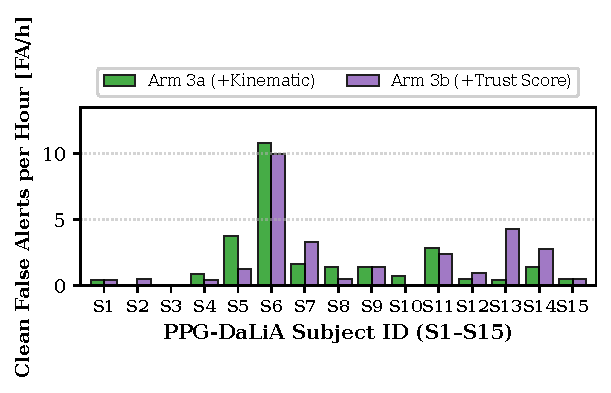
\includegraphics[width=0.98\linewidth, height=1.35in, keepaspectratio]{figures/fig_persubject_fahr.pdf}
\centerline{\footnotesize (c) Per-Subject False Alerts per Hour in Clean Data (Condition 0)}
\end{minipage}\hfill
\begin{minipage}{0.48\textwidth}
\centering
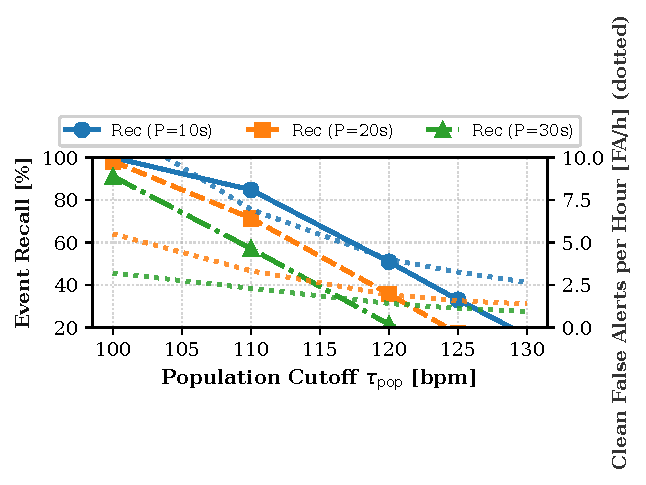
\includegraphics[width=0.98\linewidth, height=1.35in, keepaspectratio]{figures/fig_arm1_sensitivity.pdf}
\centerline{\footnotesize (d) Arm 1 Threshold Sensitivity across Cutoffs $\tau_{\text{pop}}$ and Persistence $P$}
\end{minipage}
\caption{Benchmark results across arms and conditions: (a) Event recall vs clean false alerts per hour; (b) Forest plot of paired differences ($\Delta = \text{Arm 3b} - \text{Arm 3a}$) with 95\% bootstrap CIs; (c) Per-subject FA/hr in Condition 0; (d) Arm 1 sensitivity across $\tau_{\text{pop}}$ and persistence $P$.}
\label{fig:results_all}
\end{figure*}

\section{Results and Discussion}
\subsection{Primary Hypothesis $H_1$ Outcome: NOT SUPPORTED}
Pre-registered hypothesis $H_1$ postulated that incorporating software trust scores would reduce $\text{FA/hr}$ by $\ge 60\%$ over kinematic gating and personalized baselines while preserving $\ge 85\%$ recall.

\textbf{Empirical finding: $H_1$ is not supported.} In paired per-subject comparisons (Table~\ref{tab:paired_comparison} and Fig.~\ref{fig:results_all}b), Arm 3b demonstrated no statistically detectable false-alert reduction over Arm 3a across any condition:
\begin{itemize}
    \item \textbf{Condition 0 (Clean):} Mean difference $+0.13$\,FA/h (95\% CI $[-0.54, +0.89]$, $W = 31.0$, $p = 0.8589$).
    \item \textbf{Regime A (10\% faults):} Mean difference $+0.05$\,FA/h (95\% CI $[-0.66, +0.82]$, $W = 40.0$, $p = 0.7007$).
    \item \textbf{Regime B (25--30\% faults):} Mean difference $-0.04$\,FA/h (95\% CI $[-0.78, +0.69]$, $W = 52.0$, $p = 0.9750$).
    \item \textbf{F7 (Optical Noise):} Mean difference $-0.49$\,FA/h (95\% CI $[-1.47, +0.38]$, $W = 17.0$, $p = 0.2845$).
\end{itemize}
In every condition, 95\% bootstrap confidence intervals spanned zero, and Wilcoxon tests yielded $p \ge 0.28$.

\begin{table}[htbp]
\caption{Stratified Alerting Metrics (Recall \% / FA per Hour)}
\label{tab:strata}
\centering
\tiny
\setlength{\tabcolsep}{1.8pt}
\begin{tabular}{|l|l|c|c|c|c|c|}
\hline
\textbf{Condition} & \textbf{Stratum} & \textbf{Arm 1} & \textbf{Arm 2} & \textbf{Arm 3a} & \textbf{Arm 3b} & \textbf{3b-nM} \\
\hline
Cond 0 (Clean)   & All-15      & 91\%/3.2 & 80\%/5.7 & 80\%/1.5 & 80\%/1.7 & 80\%/2.9 \\
                 & without S5  & 91\%/2.9 & 80\%/5.3 & 80\%/1.4 & 79\%/1.7 & 79\%/2.9 \\
                 & S5/6/11 (3) & 100\%/9.4 & 94\%/16.1 & 94\%/5.1 & 94\%/3.9 & 94\%/6.7 \\
\hline
Reg A (~10\%)    & All-15      & 91\%/3.6 & 80\%/6.1 & 80\%/1.6 & 80\%/1.8 & 80\%/3.1 \\
                 & without S5  & 91\%/3.3 & 80\%/5.5 & 80\%/1.4 & 79\%/1.8 & 79\%/3.0 \\
                 & S5/6/11 (3) & 100\%/9.8 & 94\%/17.1 & 94\%/5.5 & 94\%/4.1 & 94\%/7.2 \\
\hline
Reg B (~30\%)    & All-15      & 91\%/4.5 & 76\%/7.2 & 76\%/2.3 & 75\%/2.4 & 75\%/3.6 \\
                 & without S5  & 91\%/4.1 & 75\%/6.4 & 75\%/2.2 & 74\%/2.3 & 74\%/3.5 \\
                 & S5/6/11 (3) & 100\%/10.2 & 94\%/18.8 & 94\%/5.9 & 94\%/4.3 & 94\%/7.2 \\
\hline
F7 (Optical)     & All-15      & 92\%/3.1 & 64\%/4.6 & 64\%/1.6 & 58\%/1.3 & 58\%/2.0 \\
                 & without S5  & 92\%/2.7 & 63\%/4.0 & 63\%/1.2 & 56\%/1.1 & 56\%/1.9 \\
                 & S5/6/11 (3) & 100\%/9.0 & 89\%/14.9 & 89\%/5.9 & 89\%/3.5 & 89\%/5.5 \\
\hline
\end{tabular}
\end{table}

\begin{table}[htbp]
\caption{Paired Statistical Comparison: Arm 3b vs Arm 3a}
\label{tab:paired_comparison}
\centering
\scriptsize
\setlength{\tabcolsep}{2.5pt}
\begin{tabular}{lcccc}
\toprule
\textbf{Condition} & \textbf{Mean $\Delta$} & \textbf{95\% Boot. CI} & \textbf{Wilcoxon $W$} & \textbf{$p$-val} \\
\midrule
Condition 0 (Clean)    & +0.13 & [-0.54, +0.89] &  31.0 & 0.8589 \\
Regime A (~10\%)       & +0.05 & [-0.66, +0.82] &  40.0 & 0.7007 \\
Regime B (~25--30\%)   & -0.04 & [-0.78, +0.69] &  52.0 & 0.9750 \\
F7 (Optical Noise)     & -0.49 & [-1.47, +0.38] &  17.0 & 0.2845 \\
\bottomrule
\end{tabular}
\end{table}


\subsection{Secondary Benchmark Findings}
\textbf{Kinematic motion gating drives alert accuracy:} Relative to ungated Arm 2, Arm 3a reduced false alerts per hour by 74.2\% in clean data ($1.47$ vs $5.69$\,FA/h) and by 67.9\% in Regime B ($2.30$ vs $7.16$\,FA/h) (Table~\ref{tab:combined_metrics}).

\textbf{Recall degradation under optical corruption (F7):} Under intense motion-coupled optical noise, Arm 3b recall degraded to 58.0\% compared to 64.3\% in Arm 3a, indicating that multi-component software abstention can suppress genuine emergencies during noisy episodes.

\begin{table}[htbp]
\caption{Disaggregated False Alerts per Fault Type (Regimes A \& B)}
\label{tab:fault_disaggregated}
\centering
\tiny
\setlength{\tabcolsep}{1.8pt}
\begin{tabular}{llcccccc}
\toprule
\textbf{Reg.} & \textbf{Fault} & \textbf{Exp.} & \textbf{Arm 1} & \textbf{Arm 2} & \textbf{Arm 3a} & \textbf{Arm 3b} & \textbf{3b-nM} \\
\midrule
Reg A & F0\_CLEAN  & 28.1h & 3.2 (90)  & 5.9 (165) & 1.5 (43)  & 1.8 (50)  & 3.0 (83)  \\
      & F1\_GAPS   &  0.9h & 0.0 (0)*  & 0.0 (0)*  & 0.0 (0)*  & 0.0 (0)*  & 0.0 (0)*  \\
      & F2\_STALE  &  0.6h & 21.1 (13)* & 8.1 (5)*  & 3.2 (2)*  & 1.6 (1)*  & 1.6 (1)*  \\
      & F3\_DUPL   &  0.6h & 3.2 (2)*  & 8.0 (5)*  & 3.2 (2)*  & 0.0 (0)*  & 4.8 (3)*  \\
      & F4\_SPIKE  &  0.1h & 0.0 (0)*  & 14.8 (1)* & 0.0 (0)*  & 0.0 (0)*  & 14.8 (1)* \\
      & F5\_DRIFT  &  0.5h & 0.0 (0)*  & 2.2 (1)*  & 0.0 (0)*  & 0.0 (0)*  & 0.0 (0)*  \\
      & F6\_UNIT   &  0.5h & 14.5 (7)* & 26.9 (13)* & 8.3 (4)*  & 12.4 (6)* & 16.6 (8)* \\
\midrule
Reg B & F0\_CLEAN  & 21.7h & 3.5 (76)  & 5.8 (125) & 1.6 (35)  & 1.9 (40)  & 2.9 (63)  \\
      & F1\_GAPS   &  3.1h & 0.0 (0)*  & 0.0 (0)*  & 0.0 (0)*  & 0.0 (0)*  & 0.0 (0)*  \\
      & F2\_STALE  &  1.6h & 20.2 (32) & 10.8 (17) & 3.2 (5)*  & 4.4 (7)*  & 7.6 (12)  \\
      & F3\_DUPL   &  1.6h & 3.2 (5)*  & 9.6 (15)  & 1.9 (3)*  & 1.3 (2)*  & 1.9 (3)*  \\
      & F4\_SPIKE  &  0.2h & 0.0 (0)*  & 0.0 (0)*  & 0.0 (0)*  & 4.8 (1)*  & 4.8 (1)*  \\
      & F5\_DRIFT  &  1.6h & 2.6 (4)*  & 6.5 (10)  & 1.9 (3)*  & 0.7 (1)*  & 1.9 (3)*  \\
      & F6\_UNIT   &  1.6h & 15.4 (24) & 36.6 (57) & 16.7 (26) & 14.8 (23) & 19.9 (31) \\
\bottomrule
\multicolumn{8}{l}{* Insufficient data ($<10$ alerts or $<1.0$\,h). Rate shown as FA/h (count).} \\
\end{tabular}
\end{table}


\subsection{Edge-of-Grid Analysis and Fallback Rule Invocation}
Hyperparameter tuning consistently selected parameter boundary values (Table~\ref{tab:edge_of_grid}). Most notably, \textbf{Arm 2 never attained the $\ge 85\%$ recall target on any training fold in any condition} (maximum training recall achieved was $\approx 80.4\%$). Consequently, the fallback selection rule (maximizing training recall) was invoked in 100\% (15/15) of folds for Arm 2 across all regimes, selecting $k = 2.0$ and $P = 10$\,s.

\begin{table}[htbp]
\caption{Edge-of-Grid Parameter Boundary Selection Across 15 LOSO Folds}
\label{tab:edge_of_grid}
\centering
\scriptsize
\setlength{\tabcolsep}{3pt}
\begin{tabular}{|l|l|c|c|c|c|}
\hline
\textbf{Arm} & \textbf{Parameter Boundary} & \textbf{Cond 0} & \textbf{Reg A} & \textbf{Reg B} & \textbf{F7} \\
\hline
Arm 1 (Fixed)    & $\tau_{\text{pop}} = 100$\,bpm$_{\mathrm{lo}}$ & 100\% & 100\% & 100\% & 100\% \\
                 & $P = 30$\,s$_{\mathrm{hi}}$                     & 100\% & 100\% & 100\% & 100\% \\
\hline
Arm 2 (Personal) & $k = 2.0_{\mathrm{lo}}$                         & 100\% & 100\% & 100\% & 100\% \\
                 & $\kappa = 2.0$\,h$_{\mathrm{hi}}$               & 93.3\% & 93.3\% & 100\% & 100\% \\
                 & $P = 10$\,s$_{\mathrm{lo}}$                     & 100\% & 100\% & 100\% & 100\% \\
\hline
Arm 3a (+Kin.)   & $\theta_{\text{rest}} = 0.08$\,g$_{\mathrm{hi}}$ & 93.3\% & 93.3\% & 93.3\% & 100\% \\
                 & $\theta_{\text{rest}} = 0.03$\,g$_{\mathrm{lo}}$ & 6.7\%  & 6.7\%  & 6.7\%  & 0.0\% \\
\hline
Arm 3b (+Trust)  & $\theta_{\text{trust}} = 0.60_{\mathrm{lo}}$     & 93.3\% & 93.3\% & 93.3\% & 100\% \\
                 & $\theta_{\text{trust}} = 0.80_{\mathrm{hi}}$     & 6.7\%  & 6.7\%  & 6.7\%  & 0.0\% \\
\hline
\end{tabular}
\end{table}


\section{Limitations}
This benchmark is subject to several methodological constraints (Table~\ref{tab:limitations}): (1) Events were synthetically injected due to natural sparsity; (2) The cohort is limited to 15 healthy participants; (3) Algorithmic errors in front-end PPG tracking couple into downstream logic; (4) Post-result protocol amendments (Table~\ref{tab:deviations}) document adjustments made after preliminary inspection; (5) Arm 4 (conformal prediction with selective abstention) was never built or evaluated; (6) PhysioNet Wearable 1.0.1 and WESAD \cite{ref_wesad} datasets were not used for benchmark evaluation, maintaining focus strictly on the ratified PPG-DaLiA protocol.

\begin{table}[htbp]
\caption{Threats to Validity and Scientific Limitations}
\label{tab:limitations}
\centering
\scriptsize
\begin{tabular}{lp{4.7cm}}
\toprule
\textbf{Threat Domain} & \textbf{Empirical Limitation and Mitigation} \\
\midrule
Synthetic Events & True resting tachycardia was absent in healthy cohort; 112 episodes synthetically injected into derived stream. Recall values are tied to synthetic plateau distribution ($105$--$135$\,bpm). \\
Cohort Size & $N = 15$ healthy young adults limits power for small paired false-alert differences. Reported with 95\% bootstrap CIs. \\
Noise Coupling & Estimator tracking errors and motion artifacts interact directly with downstream thresholding logic. \\
Grid Boundaries & Tuning frequently selected grid boundaries ($\tau_{\text{pop}} = 100$, $k = 2.0$, $P = 10$\,s / $30$\,s), reflecting severe trade-offs. \\
Ambulatory Protocol & Single 2.5-hour multimodal script; generalizability to continuous free-living 24/7 monitoring is not established. \\
Non-Clinical Scope & Academic software benchmark only; not validated for clinical diagnosis or medical device deployment. \\
\bottomrule
\end{tabular}
\end{table}

\begin{table}[htbp]
\caption{Protocol Evolution and Amendments (from git log)}
\label{tab:deviations}
\centering
\scriptsize
\begin{tabular}{lp{4.7cm}}
\toprule
\textbf{Milestone [Commit]} & \textbf{Ratified Scope and Description} \\
\midrule
Protocol v1.0.0 [\texttt{41eff1e}] & Frozen protocol: $H_1$--$H_3$, faults F1--F7, LOSO cross-validation. \\
Amendment 1 [\texttt{3b1f2f6}] & Resting alert ground truth; non-penalization of motion. \\
Implementation Fix [\texttt{3a5ccc2}] & Removed $/64$ accel scaling; centered 8\,s windows ($t=2i+4$\,s). \\
Amendment 2 [\texttt{696fd00}] & Labelled synthetic tachycardia injection; S5 outlier handling rule. \\
Adaptive Ramp Fix [\texttt{a0d682a}] & Baseline-adapted ramp rates ($r_{\text{lo}}, r_{\text{hi}}$); plateau $[105, 135]$\,bpm. \\
Amendment 3 [\texttt{a0d682a}] & Restated $H_1$ as estimation; 15-subject LOSO; Arm 3b-noMotion ablation. \\
Gap Enforcement [\texttt{0bf4ca4}] & Ratified 112 episodes with $\ge 60$\,s minimum inter-episode gap. \\
Amendment 4 [\texttt{a9ce657}] & Standard emitter: $P \in \{10,20,30\}$\,s, $R=60$\,s; parameter grids. \\
Fallback Rule [\texttt{f92ca8d}] & Arm 2 fallback invoked in 100\% of folds (max recall $\approx 80.4\% < 85\%$). \\
\bottomrule
\end{tabular}
\end{table}


\section{Future Scope}
Future efforts will extend this benchmark along five technical avenues:
\begin{enumerate}
    \item \textbf{Arm 4 Conformal Abstention:} Building and integrating inductive conformal prediction to yield distribution-free validity sets with user-calibrated error bounds \cite{ref_vazquez_conformal}.
    \item \textbf{External Dataset Generalization:} Evaluating on external public wearable corpora, including the PhysioNet Wearable Device Dataset \cite{ref_physionet_wearable} and WESAD \cite{ref_wesad}.
    \item \textbf{Clinical Patient Cohorts:} Validating on holter-monitored inpatient recordings with spontaneous atrial fibrillation and supraventricular tachycardia.
    \item \textbf{On-Device Hardware Integration:} Deploying causal baseline and kinematic gating engines onto low-power embedded microcontrollers.
    \item \textbf{Symptom-Risk Questionnaire Module:} Implementing PRD modules FR-06 (guided questionnaire) and FR-07 (explanation and uncertainty) to complement passive telemetry.
\end{enumerate}

\section{Conclusion}
In this pre-registered fault-injection benchmark, kinematic motion gating accounted for virtually all false-alert suppression in wearable heart-rate monitoring, while multi-component software trust scoring offered no statistically detectable benefit. Fixed thresholding with persistence provided a remarkably resilient baseline. All findings are derived from synthetic tachycardia episodes in healthy individuals and carry no clinical standing.

\section*{Regulatory and Safety Statement}
\textbf{Not a Medical Device:} The VitaSense AI software, alerting algorithms, and benchmark suite are academic research artifacts. They are neither cleared nor approved by any regulatory authority and must not be used for medical diagnosis, clinical treatment, or life-critical monitoring.

\section*{Data and Code Availability}
The PPG-DaLiA dataset is openly accessible via the UCI Machine Learning Repository \cite{ref_reiss_dalia, ref_uci_dalia}. The PhysioNet Wearable Device Dataset is available under ODC-By v1.0 \cite{ref_physionet_wearable}. Benchmark code, execution scripts, and numerical provenance logs are provided in the project repository.

\begin{thebibliography}{00}

% URL: https://www.ncbi.nlm.nih.gov/pmc/articles/PMC6679242/
% Accessed: 2026-10-22
\bibitem{ref_reiss_dalia}
A.~Reiss, I.~Indlekofer, P.~Schmidt, and K.~Van~Laerhoven, ``Deep PPG: Large-scale heart rate estimation with convolutional neural networks,'' \emph{Sensors}, vol.~19, no.~14, p.~3079, 2019.

% URL: https://www.ncbi.nlm.nih.gov/pmc/articles/PMC5597264/
% Accessed: 2026-10-22
\bibitem{ref_elgendi_sqi}
M.~Elgendi, ``Optimal signal quality index for photoplethysmogram signals,'' \emph{Bioengineering}, vol.~3, no.~4, p.~21, 2016.

% URL: https://www.ncbi.nlm.nih.gov/pmc/articles/PMC10686289/
% Accessed: 2026-10-22
\bibitem{ref_charlton_roadmap}
P.~H.~Charlton \emph{et al.}, ``The 2023 wearable photoplethysmography roadmap,'' \emph{Journal of Physics: Photonics}, vol.~5, no.~4, p.~042501, 2023.

% URL: https://www.ncbi.nlm.nih.gov/pmc/articles/PMC9309105/
% Accessed: 2026-10-22
\bibitem{ref_vazquez_conformal}
J.~Vazquez and J.~C.~Facelli, ``Conformal prediction in clinical medical sciences,'' \emph{Journal of Healthcare Informatics Research}, vol.~6, no.~3, pp.~257--285, 2022.

% URL: https://archive.ics.uci.edu/dataset/495/ppg+dalia
% Accessed: 2026-10-22
\bibitem{ref_uci_dalia}
A.~Reiss, I.~Indlekofer, P.~Schmidt, and K.~Van~Laerhoven, ``PPG-DaLiA,'' UCI Machine Learning Repository, 2019, DOI: 10.24432/C53890.

% URL: https://archive.ics.uci.edu/dataset/45/heart+disease
% Accessed: 2026-10-22
\bibitem{ref_uci_heart}
R.~Detrano, A.~J\'anosi, W.~Steinbrunn, K.~Pfisterer, and J.~Schmid, ``Heart Disease,'' UCI Machine Learning Repository, 1988, DOI: 10.24432/C52P4X.

% URL: https://physionet.org/content/wearable-device-dataset/1.0.1/
% Accessed: 2026-10-22
\bibitem{ref_physionet_wearable}
A.~Kos, Y.~Toma\v{z}i\v{c}, and A.~Umek, ``Wearable Device Dataset from Induced Stress and Structured Exercise Sessions,'' PhysioNet, Version 1.0.1, 2022, DOI: 10.13026/8fca-2v93.

% URL: https://dl.acm.org/doi/10.1145/3242969.3242985
% Accessed: 2026-10-22
\bibitem{ref_wesad}
P.~Schmidt, A.~Reiss, R.~Duerichen, C.~Marberger, and K.~Van~Laerhoven, ``Introducing WESAD, a multimodal dataset for wearable stress and affect detection,'' in \emph{Proc. 20th ACM Int. Conf. Multimodal Interaction (ICMI)}, 2018, pp.~400--408.

% URL: https://ieeexplore.ieee.org/document/6905807
% Accessed: 2026-10-22
\bibitem{ref_troika}
Z.~Zhang, Z.~Pi, and B.~Liu, ``TROIKA: A general framework for heart rate monitoring using wrist-type photoplethysmographic signals during intensive physical exercise,'' \emph{IEEE Trans. Biomed. Eng.}, vol.~62, no.~2, pp.~522--531, 2015.

% URL: https://pubmed.ncbi.nlm.nih.gov/22614385/
% Accessed: 2026-10-22
\bibitem{ref_alarm_fatigue}
M.~Cvach, ``Monitor alarm fatigue: An integrative review,'' \emph{Biomed. Instrum. Technol.}, vol.~46, no.~4, pp.~268--277, 2012.

\end{thebibliography}

\end{document}
